\documentclass[10pt]{article}
\usepackage[letterpaper]{geometry}
\geometry{verbose,tmargin=1in,bmargin=1in,lmargin=1in,rmargin=1in}
\usepackage{setspace}
\usepackage{ragged2e}
\usepackage{color}
\usepackage{titlesec}
\usepackage{graphicx}
\usepackage{float}
\usepackage{mathtools}
\usepackage{amsmath}
\usepackage[font=small,labelfont=bf,labelsep=period]{caption}
\usepackage[english]{babel}
\usepackage{indentfirst}
\usepackage{array}
\usepackage{makecell}
\usepackage[usenames,dvipsnames]{xcolor}
\usepackage{multirow}
\usepackage{tabularx}
\usepackage{arydshln}
\usepackage{caption}
\usepackage{subcaption}
\usepackage{xfrac}
\usepackage{etoolbox}
\usepackage{cite}
\usepackage{url}
\usepackage{dcolumn}
\usepackage{hyperref}
\usepackage{courier}
\usepackage{url}
\usepackage{esvect}
\usepackage{commath}
\usepackage{verbatim} % for block comments
\usepackage{enumitem}
\usepackage{hyperref} % for clickable table of contents
\usepackage{braket}
\usepackage{titlesec}
\usepackage{booktabs}
\usepackage{gensymb}
\usepackage{longtable}
\usepackage{soul} % for striking out text
\usepackage[makeroom]{cancel}	% to cancel out text

\usepackage{listings}
\lstset{
    frame=single,
    breaklines=true,
    postbreak=\raisebox{0ex}[0ex][0ex]{\ensuremath{\color{red}\hookrightarrow\space}}
}

% for circled numbers
\usepackage{tikz}
\newcommand*\circled[1]{\tikz[baseline=(char.base)]{
            \node[shape=circle,draw,inner sep=2pt] (char) {#1};}}


\titleclass{\subsubsubsection}{straight}[\subsection]

% define new command for triple sub sections
\newcounter{subsubsubsection}[subsubsection]
\renewcommand\thesubsubsubsection{\thesubsubsection.\arabic{subsubsubsection}}
\renewcommand\theparagraph{\thesubsubsubsection.\arabic{paragraph}} % optional; useful if paragraphs are to be numbered

\titleformat{\subsubsubsection}
  {\normalfont\normalsize\bfseries}{\thesubsubsubsection}{1em}{}
\titlespacing*{\subsubsubsection}
{0pt}{3.25ex plus 1ex minus .2ex}{1.5ex plus .2ex}

\makeatletter
\renewcommand\paragraph{\@startsection{paragraph}{5}{\z@}%
  {3.25ex \@plus1ex \@minus.2ex}%
  {-1em}%
  {\normalfont\normalsize\bfseries}}
\renewcommand\subparagraph{\@startsection{subparagraph}{6}{\parindent}%
  {3.25ex \@plus1ex \@minus .2ex}%
  {-1em}%
  {\normalfont\normalsize\bfseries}}
\def\toclevel@subsubsubsection{4}
\def\toclevel@paragraph{5}
\def\toclevel@paragraph{6}
\def\l@subsubsubsection{\@dottedtocline{4}{7em}{4em}}
\def\l@paragraph{\@dottedtocline{5}{10em}{5em}}
\def\l@subparagraph{\@dottedtocline{6}{14em}{6em}}
\makeatother

\newcommand{\volume}{\mathop{\ooalign{\hfil$V$\hfil\cr\kern0.08em--\hfil\cr}}\nolimits}

\setcounter{secnumdepth}{4}
\setcounter{tocdepth}{4}
\begin{document}

\textbf{NE 255: HW3}2, 4\hfill April Novak\newline

\circled{1} Due to the added complexity associated with higher dimensions, the \(P_N\) equations are derived here for the time-independent form of the 1-D, monoenergetic transport equation in Cartesian geometries given by the following equation, where the external and fission source are bundled together into \(S\), which is assumed isotropic:

\begin{equation*}
\mu \frac{\partial \psi(z, \mu)}{\partial z} +
 \Sigma_t(z)\psi(z, \mu) =\int_{4\pi}^{} d\hat{\Omega}' \Sigma_s(z, \hat{\Omega}\cdot\hat{\Omega}')\psi(z,\hat{\Omega}') + \frac{S(z)}{4\pi}
 \end{equation*}

After the \(P_N\) equations are derived for this equation, then the extension to the \(SP_N\) equations will be performed using heuristic arguments, although with much more effort, you could show that the \(SP_N\) equations are an asymptotic solution to the transport equation. The \(P_N\) approximation is made by expanding both the flux and scattering cross section in Legendre polynomials. We use Legendre polynomials here because we're in 1-D Cartesian geometry; in higher dimensions or in non-Cartesian frames, the spherical harmonics would be needed.

\begin{equation}
\label{eq:AngularFluxPN}
\psi(z,\mu)=\sum_{n=0}^{\infty}\frac{2n+1}{4\pi}\phi_n(z)P_n(\mu)
\end{equation}

\begin{equation}
\label{eq:PNScatteringCrossSectionExpansion}
\Sigma_s(z,\hat{\Omega}\cdot\hat{\Omega}')=\sum_{l=0}^{\infty}\frac{2l+1}{4\pi}\Sigma_{sl}(z)P_l(\hat{\Omega}\cdot\hat{\Omega}')\rightarrow\sum_{l=0}^{\infty}\frac{2l+1}{4\pi}\Sigma_{sl}(z)P_l(\mu)P_l(\mu')
\end{equation}

where \(n\) is used in the expansion of the flux to differentiate it from \(l\) used in expanding the scattering cross section. From the 1-D form of the addition theorem for spherical harmonics, the scattering cross section expansion has been simplified. Now, inserting Eqs. \eqref{eq:AngularFluxPN} and \eqref{eq:AngularFluxPN} into the 1-D transport equation listed in the beginning of this section:

\begin{equation}
\begin{aligned}
\mu \frac{\partial}{\partial z}\left(\sum_{n=0}^{\infty}\frac{2n+1}{4\pi}\phi_n(z)P_n(\mu)\right) + \Sigma_t(z)\sum_{n=0}^{\infty}\frac{2n+1}{4\pi}\phi_n(z)P_n(\mu) =\quad\quad\\
\int_{4\pi}^{} d\hat{\Omega}' \sum_{l=0}^{\infty}\frac{2l+1}{4\pi}\Sigma_{sl}(z)P_l(\mu)P_l(\mu')\sum_{n=0}^{\infty}\frac{2n+1}{4\pi}\phi_n(z)P_n(\mu) + \frac{S(z)}{4\pi}
 \end{aligned}
 \end{equation}

Because no quantities depend on \(\hat{\Omega}\), the scattering integral can be integrated over \(0\leq\phi\leq2\pi\) so that the integral becomes a function of only \(\mu\) and space.

\begin{equation}
\label{eq:PNStep1}
\begin{aligned}
\mu \frac{\partial}{\partial z}\left(\sum_{n=0}^{\infty}\frac{2n+1}{4\pi}\phi_n(z)P_n(\mu)\right) + \Sigma_t(z)\sum_{n=0}^{\infty}\frac{2n+1}{4\pi}\phi_n(z)P_n(\mu) =\quad\quad\\
2\pi\int_{-1}^{1} d\mu' \sum_{l=0}^{\infty}\frac{2l+1}{4\pi}\Sigma_{sl}(z)P_l(\mu)P_l(\mu')\sum_{n=0}^{\infty}\frac{2n+1}{4\pi}\phi_n(z)P_n(\mu) + \frac{S(z)}{4\pi}
 \end{aligned}
 \end{equation}
 
The orthogonality property of Legendre polynomials does not permit any extra terms (that depend on \(\mu\)) to be present in the integrand. Hence, the first term in Eq. \eqref{eq:PNStep1} must be rewritten using the recursive property of Legendre polynomials:

 \begin{equation}
\label{eq:PNStep2}
\begin{aligned}
\frac{\partial}{\partial z}\left(\sum_{n=0}^{\infty}\frac{\cancel{2n+1}}{4\pi}\phi_n(z)\frac{1}{\cancel{2n+1}} \left\lbrack(n+1)P_{n+1}(\mu) + n P_{n-1}(\mu)\right\rbrack\right) + \Sigma_t(z)\sum_{n=0}^{\infty}\frac{2n+1}{4\pi}\phi_n(z)P_n(\mu) =\quad\quad\\
2\pi\int_{-1}^{1} d\mu' \sum_{l=0}^{\infty}\frac{2l+1}{4\pi}\Sigma_{sl}(z)P_l(\mu)P_l(\mu')\sum_{n=0}^{\infty}\frac{2n+1}{4\pi}\phi_n(z)P_n(\mu) + \frac{S(z)}{4\pi}
 \end{aligned}
 \end{equation}
 
 Multiplying Eq. \eqref{eq:PNStep2} by \(P_n(\mu)\) and then integrating over \(-1\leq\mu\leq1\) gives, after canceling the \(1/4\pi\) from each term:
 
  \begin{equation}
\label{eq:PNStep3}
\begin{aligned}
\frac{\partial}{\partial z}\left(\sum_{n=0}^{\infty}\left\lbrack\int_{-1}^{1}d\mu\phi_n(z)(n+1)P_{n+1}(\mu)P_n(\mu) + \int_{-1}^{1}d\mu\phi_n(z)n P_{n-1}(\mu)P_n(\mu)\right\rbrack\right) + \quad\quad\\
\Sigma_t(z)\sum_{n=0}^{\infty}(2n+1)\int_{-1}^{1}d\mu\phi_n(z)P_n(\mu)P_n(\mu) =\quad\quad\\
\int_{-1}^{1}d\mu P_n(\mu)2\pi\int_{-1}^{1} d\mu' \sum_{l=0}^{\infty}\frac{2l+1}{4\pi}\Sigma_{sl}(z)P_l(\mu)P_l(\mu')\sum_{n=0}^{\infty}(2n+1)\phi_n(z)P_n(\mu)P_n(\mu) + \int_{-1}^{1}d\mu S(z)P_n(\mu)
 \end{aligned}
 \end{equation}

Then, applying the orthogonality property of Legendre polynomials gives:

  \begin{equation}
\label{eq:PNStep4}
\begin{aligned}
\frac{\partial}{\partial z}\left(\sum_{n=0}^{\infty}\left\lbrack\frac{2(n+1)}{2n+1}\phi_{n+1}(z) +\frac{2n}{2n+1} \phi_{n-1}(z)\right\rbrack\right) + \Sigma_t(z)\sum_{n=0}^{\infty}2\phi_n(z) =\quad\quad\\
2\sum_{l=0}^{\infty}\Sigma_{sl}(z)\sum_{n=0}^{\infty}\phi_n(z) + \int_{-1}^{1}d\mu S(z)P_n(\mu)
 \end{aligned}
 \end{equation}

where orthogonality was applied twice to the scattering term. Dividing through by 2 then gives the \(P_N\) equations for 1-D Cartesian geometries:

\begin{equation}
\label{eq:PNStep5}
\begin{aligned}
\frac{\partial}{\partial z}\left(\sum_{n=0}^{\infty}\left\lbrack\frac{n+1}{2n+1}\phi_{n+1}(z) +\frac{n}{2n+1} \phi_{n-1}(z)\right\rbrack\right) + \Sigma_t(z)\sum_{n=0}^{\infty}\phi_n(z) =\quad\quad\\
\sum_{l=0}^{\infty}\Sigma_{sl}(z)\sum_{n=0}^{\infty}\phi_n(z) + \delta_{n,even}\frac{1}{2}\int_{-1}^{1}d\mu S(z)P_n(\mu)
 \end{aligned}
 \end{equation}

Because \(S(z)\) is not a function of \(\mu\), then the integral of a Legendre polynomial over its basis will give zero if that Legendre polynomial is an odd function, and will be nonzero otherwise. Hence, the source term is only present for even \(n\), based on the form of the Legendre polynomials. For odd-\(n\), the Legendre polynomials contain a sum of odd functions, and the integral of any odd function over a region symmetric about the origin is zero. Now, in order to make this solution method tractable, the infinite sums have to be truncated at some point. It is also customary to set \(l=n\) such that the above reduce to:

\begin{equation}
\label{eq:PNStep6}
\begin{aligned}
\frac{\partial}{\partial z}\left(\sum_{n=0}^{N}\left\lbrack\frac{n+1}{2n+1}\phi_{n+1}(z) +\frac{n}{2n+1} \phi_{n-1}(z)\right\rbrack\right) + \Sigma_t(z)\sum_{n=0}^{N}\phi_n(z) =\quad\quad\\
\sum_{n=0}^{N}\Sigma_{sn}(z)\phi_n(z) +  \delta_{n,even}\frac{1}{2}\int_{-1}^{1}d\mu S(z)P_n(\mu)
 \end{aligned}
 \end{equation}

We can require Eq. \eqref{eq:PNStep6} to hold for all \(N\) at once, but we can also require it to hold for each \(N\). This stricter requirement returns the requirement stated in Eq. \eqref{eq:PNStep6}, and hence the \(P_N\) equations in practice produce \(N\) coupled ODEs:

\begin{equation}
\label{eq:PNEquations}
\begin{aligned}
\frac{\partial}{\partial z}\left\lbrack\frac{n+1}{2n+1}\phi_{n+1}(z) +\frac{n}{2n+1} \phi_{n-1}(z)\right\rbrack + \Sigma_t(z)\phi_n(z) =
\Sigma_{sn}(z)\phi_n(z) +  \delta_{n,even}\frac{1}{2}\int_{-1}^{1}d\mu S(z)P_n(\mu)
 \end{aligned}
 \end{equation}

This gives \(N+1\) coupled equations. For example, some of the first \(P_N\) equations are:
 
 \begin{equation}
 \begin{aligned}
\frac{\partial\phi_{1}(z)}{\partial z} + \Sigma_t(z)\phi_0(z)=\Sigma_{s0}\phi_0(z)+ S_0(z)\quad\quad n=0\\
\frac{2}{3}\frac{\partial\phi_{2}(z)}{\partial z}+\frac{1}{3}\frac{\partial\phi_{0}(z)}{\partial z} + \Sigma_t(z)\phi_1(z)=\Sigma_{s1}\phi_1(z)\quad\quad n=1\\
\frac{3}{5}\frac{\partial\phi_{3}(z)}{\partial z}+\frac{2}{5}\frac{\partial\phi_{1}(z)}{\partial z} + \Sigma_t(z)\phi_2(z)=\Sigma_{s2}\phi_2(z)+ S_2(z)\quad\quad n=2\\
\end{aligned}
\end{equation}

In order to truncate the infinite series to \(N\) unknowns, \(\phi_{-1}=0\) is often set, and either \(\phi_{N+1}=0\) or \(\partial\phi_{N+1}/\partial z=0\) is set as the other condition, where both give equivalent results. \(N\) is usually selected to be odd. If \(N\) were even, then artificial symmetry would be introduced into the problem through application of boundary conditions. In addition, for even \(N\), you do not obtain any additional information (non-linearly independent) from the \(P_N\) equations.

A heuristic derivation of the \(SP_N\) equations can be performed using simple arguments regarding the form of the 1-D \(P_N\) equations in Eq. \eqref{eq:PNEquations}. The key to deriving the \(SP_N\) equations is to transform Eq. \eqref{eq:PNEquations} such that the derivative in the even-\(n\) equations is replaced by a divergence, while the derivative in the odd-\(n\) equations is replaced by a gradient. The \(SP_N\) equations therefore are:

\begin{equation}
\label{eq:SPNEquations}
\begin{aligned}
\frac{n+1}{2n+1}\nabla\cdot\vv{\phi}_{n+1}(z)+\frac{n}{2n+1}\nabla\cdot\vv{\phi}_{n-1}(z)+ \Sigma_t(z)\phi_n(z)=\Sigma_{sn}\phi_n(z)+ S_n(z)\quad \textrm{even - } n\\
\frac{n+1}{2n+1}\nabla\phi_{n+1}(z)+\frac{n}{2n+1}\nabla\phi_{n-1}(z)+ \Sigma_t(z)\vv{\phi}_n(z)=\Sigma_{sn}\vv{\phi}_n(z)\quad \textrm{odd - } n\\
\end{aligned}
 \end{equation}

This first-order form gives \(N+1\) equations. The \(SP_N\) equations can also be written in second-order form by solving for the odd moments in the odd-\(n\) equations, and then substituting this into the even moment equations. The \(SP_5\) equations are therefore:

\begin{equation}
\begin{aligned}
\nabla\cdot\vv{\phi}_{1}(z)+ \Sigma_t(z)\phi_0(z)=\Sigma_{s0}\phi_0(z)+ S_0(z)\quad n=0\\
\frac{2}{3}\nabla\phi_{2}(z)+\frac{1}{3}\nabla\phi_{0}(z)+ \Sigma_t(z)\vv{\phi}_1(z)=\Sigma_{s1}\vv{\phi}_1(z)\quad n=1\\
\frac{3}{5}\nabla\cdot\vv{\phi}_{3}(z)+\frac{2}{5}\nabla\cdot\vv{\phi}_{1}(z)+ \Sigma_t(z)\phi_2(z)=\Sigma_{s2}\phi_2(z)+ S_2(z)\quad n=2\\
\frac{4}{7}\nabla\phi_{4}(z)+\frac{3}{7}\nabla\phi_{2}(z)+ \Sigma_t(z)\vv{\phi}_3(z)=\Sigma_{s3}\vv{\phi}_3(z)\quad n=3\\
\frac{5}{9}\nabla\cdot\vv{\phi}_{5}(z)+\frac{4}{9}\nabla\cdot\vv{\phi}_{3}(z)+ \Sigma_t(z)\phi_4(z)=\Sigma_{s4}\phi_4(z)+ S_4(z)\quad n=4\\
\frac{6}{11}\nabla\phi_{6}(z)+\frac{5}{11}\nabla\phi_{4}(z)+ \Sigma_t(z)\vv{\phi}_5(z)=\Sigma_{s5}\vv{\phi}_5(z)\quad n=5\\
\end{aligned}
\end{equation}

If we assume an isotropic source, then \(S_n=0\) for \(n\neq0\). This simplifies the above to:

\begin{equation}
\begin{aligned}
\nabla\cdot\vv{\phi}_{1}(z)+ \Sigma_t(z)\phi_0(z)=\Sigma_{s0}\phi_0(z)+ S_0(z)\quad n=0\\
\frac{2}{3}\nabla\phi_{2}(z)+\frac{1}{3}\nabla\phi_{0}(z)+ \Sigma_t(z)\vv{\phi}_1(z)=\Sigma_{s1}\vv{\phi}_1(z)\quad n=1\\
\frac{3}{5}\nabla\cdot\vv{\phi}_{3}(z)+\frac{2}{5}\nabla\cdot\vv{\phi}_{1}(z)+ \Sigma_t(z)\phi_2(z)=\Sigma_{s2}\phi_2(z)\quad n=2\\
\frac{4}{7}\nabla\phi_{4}(z)+\frac{3}{7}\nabla\phi_{2}(z)+ \Sigma_t(z)\vv{\phi}_3(z)=\Sigma_{s3}\vv{\phi}_3(z)\quad n=3\\
\frac{5}{9}\nabla\cdot\vv{\phi}_{5}(z)+\frac{4}{9}\nabla\cdot\vv{\phi}_{3}(z)+ \Sigma_t(z)\phi_4(z)=\Sigma_{s4}\phi_4(z)\quad n=4\\
\frac{6}{11}\nabla\phi_{6}(z)+\frac{5}{11}\nabla\phi_{4}(z)+ \Sigma_t(z)\vv{\phi}_5(z)=\Sigma_{s5}\vv{\phi}_5(z)\quad n=5\\
\end{aligned}
\end{equation}

For vacuum boundary conditions, we set Marshak boundary conditions on the odd flux moments. 

\begin{equation}
2\pi\int_{\hat{\Omega}\cdot\hat{n}<0}^{}d\mu P_l(\mu)\psi(\mu)=2\mu\int_{\hat{\Omega}\cdot\hat{n}<0}^{}d\mu P_l(\mu)\psi_b(\mu)\quad\quad l=1, 3, 5\cdots N
\end{equation}

where \(\psi_b=0\) because for vacuum boundaries we assume no incoming flux. Then, to be explicit, the boundary conditions listed above become:

\begin{equation}
\begin{aligned}
2\pi\int_{\hat{\Omega}\cdot\hat{n}<0}^{}d\mu P_1(\mu)\psi(\mu)=0\quad\rightarrow\quad \phi_1(\mu)=0, \mu<0 \textrm{(incoming)}\\
2\pi\int_{\hat{\Omega}\cdot\hat{n}<0}^{}d\mu P_3(\mu)\psi(\mu)=0\quad\rightarrow\quad \phi_3(\mu)=0, \mu<0 \textrm{(incoming)}\\
2\pi\int_{\hat{\Omega}\cdot\hat{n}<0}^{}d\mu P_5(\mu)\psi(\mu)=0\quad\rightarrow\quad \phi_5(\mu)=0, \mu<0 \textrm{(incoming)}\\
\end{aligned}
\end{equation}

\circled{2} (a) The following integral will be evaluated using the \(LQ_N\) quadrature rules:

\begin{equation}
\label{eq:Sn}
\int_{4\pi}^{}d\hat{\Omega}|\hat{\Omega}|=\int_{4\pi}^{}d\hat{\Omega}\sqrt{(\xi^2+\eta^2+\mu^2)}=8\sum_{i=1}^{N(N+2)/8}w_i\sqrt{(\xi_i^2+\eta_i^2+\mu_i^2)}
\end{equation}

where

\begin{equation}
\hat{\Omega}=\xi\hat{x}_1+\eta\hat{x}_2+\mu\hat{x}_3
\end{equation}

However, the integration in Eq. \eqref{eq:Sn} assumes that the weights are normalized such that integration over the entire unit sphere gives unity. This quadrature rule is designed such that it is normalized over a single octant. Over an octant, \(\mu\) ranges from 0 to 1 and \(\phi\)from 0 to \(\pi/2\). Hence, the end result of the integration with the quadrature rules from Lewis and Miller must be multiplied by \(2/\pi\) to attain the correct normalization. The Appendix contains the code used for this section. Using the \(S_4\) \(LQ_N\) quadrature, integration over the unit sphere gives a value of \(4\pi\), which is expected analytically. Because the quadrature points are all on the unit sphere, the integrand in Eq. \eqref{eq:Sn} can be exactly integrated with the level-symmetric quadrature.\newline

(b) With \(S_6\) quadrature, a value of \(4\pi\) is again obtained. Hence, for this simple integration, again because all quadrature points already lie on the unit sphere, this integral can be exactly integrated.\newline

(c) 




\circled{3} (a) \underline{Complexity}: In terms of complexity, deterministic methods are the most difficult to derive, understand, and encode. Diffusion theory is a deterministic method, and because it consists of one equation (assuming there is no anisotropic source, and that the time rate of change of the current with respect to its magnitude is small), it is not very complex to understand or encode. Diffusive equations also have very nice numerical properties, and do not require the messy stabilization methods required for nonlinear physics such as the Navier-Stokes equations. Deterministic methods require procedures for discretizing in space, angle, energy, and time, while this is not required of Monte Carlo methods. The Monte Carlo code Serpent, for instance, is continuous in all of these variables except time, but finite differencing time stepping is only performed in the depletion subroutines (I think?). Monte Carlo methods are the least complex because they require simply tracking particle motion around repeatedly, though they can become complex once weight windows and particle tracking are introduced to improve the statistics.\newline

\underline{Accuracy}: Without the restrictions of computational cost, Monte Carlo methods are the most accurate, since there is no ``approximation'' of the physics or numerical errors that are always present in deterministic methods. For instance, in deterministic methods, there is always some type of truncation error that is present due to approximating a continuous process over a discrete mesh. In general, transport solutions are more accurate than diffusive solutions provided that the transport solutions were not performed with such a poor mesh that they are ``useless.'' However, the benefit of deterministic methods is that they can potentially be more accurate than Monte Carlo solutions when constrained to a fixed run time, especially for shielding problems where a very large number of particles would need to be run in order to obtain sufficient statistics.\newline

\underline{Run time}: It is difficult to rank these methods in terms of run time, since increasing the number of particles or refining the mesh can always lead to a higher run time. To obtain the same level of error, I cannot say beforehand which method, deterministic or Monte Carlo, could obtain the result faster. If someone knew then we might not be studying one of the methods entirely! Diffusion problems will most likely run much faster than Monte Carlo and other deterministic methods. Deterministic methods on average likely run faster than Monte Carlo problems, since, especially for large geometries, Monte Carlo simulations can require very many particles to obtain satisfactory statistics.\newline

\underline{Applicability}: When using the diffusion equations, you are inherently assuming that 1) the angular flux is at most linearly anisotropic, 2) the time rate of change of the current is small with respect to its magnitude, and 3) there is no anisotropic source. Diffusion theory breaks down when the medium becomes poorly-scattering, i.e. near strong absorbers, near void regions or vacuum boundaries, and near material interfaces with strong changes in cross section. Due to the high level of generality of Monte Carlo methods, they are applicable under all situations that are governed by stochastic processes. Assuming that nuclear interactions are always stochastic, then Monte Carlo methods are applicable so long as the underlying nuclear data is accurate. Deterministic methods often place limitations of the degree of angular discretization, so for highly-dependent angular solutions, it may be better to use a Monte Carlo solution instead of a deterministic method with an unknown mesh requirement.\newline

(b) \underline{Some strengths of deterministic methods include}:

\begin{enumerate}
\item Generally have lower run times than Monte Carlo methods
\item Accuracy is always the same (i.e. you don't need to re-run the simulation many times to obtain an averaged result)
\item More closely related to transport theory, so interesting academic and mathematical results can be derived to inspire new methods
\end{enumerate} 

\underline{Some weaknesses of deterministic methods include}:

\begin{enumerate}
\item More difficult to program and understand as a general user than Monte Carlo codes
\item Mesh refinement studies have to be performed before being able to trust the results
\item You always need to check that the range of validity of the equations fits your application before using a deterministic code
\end{enumerate}

\clearpage
\circled{4} (a) Figures \ref{fig:real} and \ref{fig:imag} plot the real and imaginary components of \(Y_{lm}\) for \(l=0, 1, 2\) and for \(-l\leq m\leq l\).
\begin{comment}
\begin{figure}[H]
  \centering
  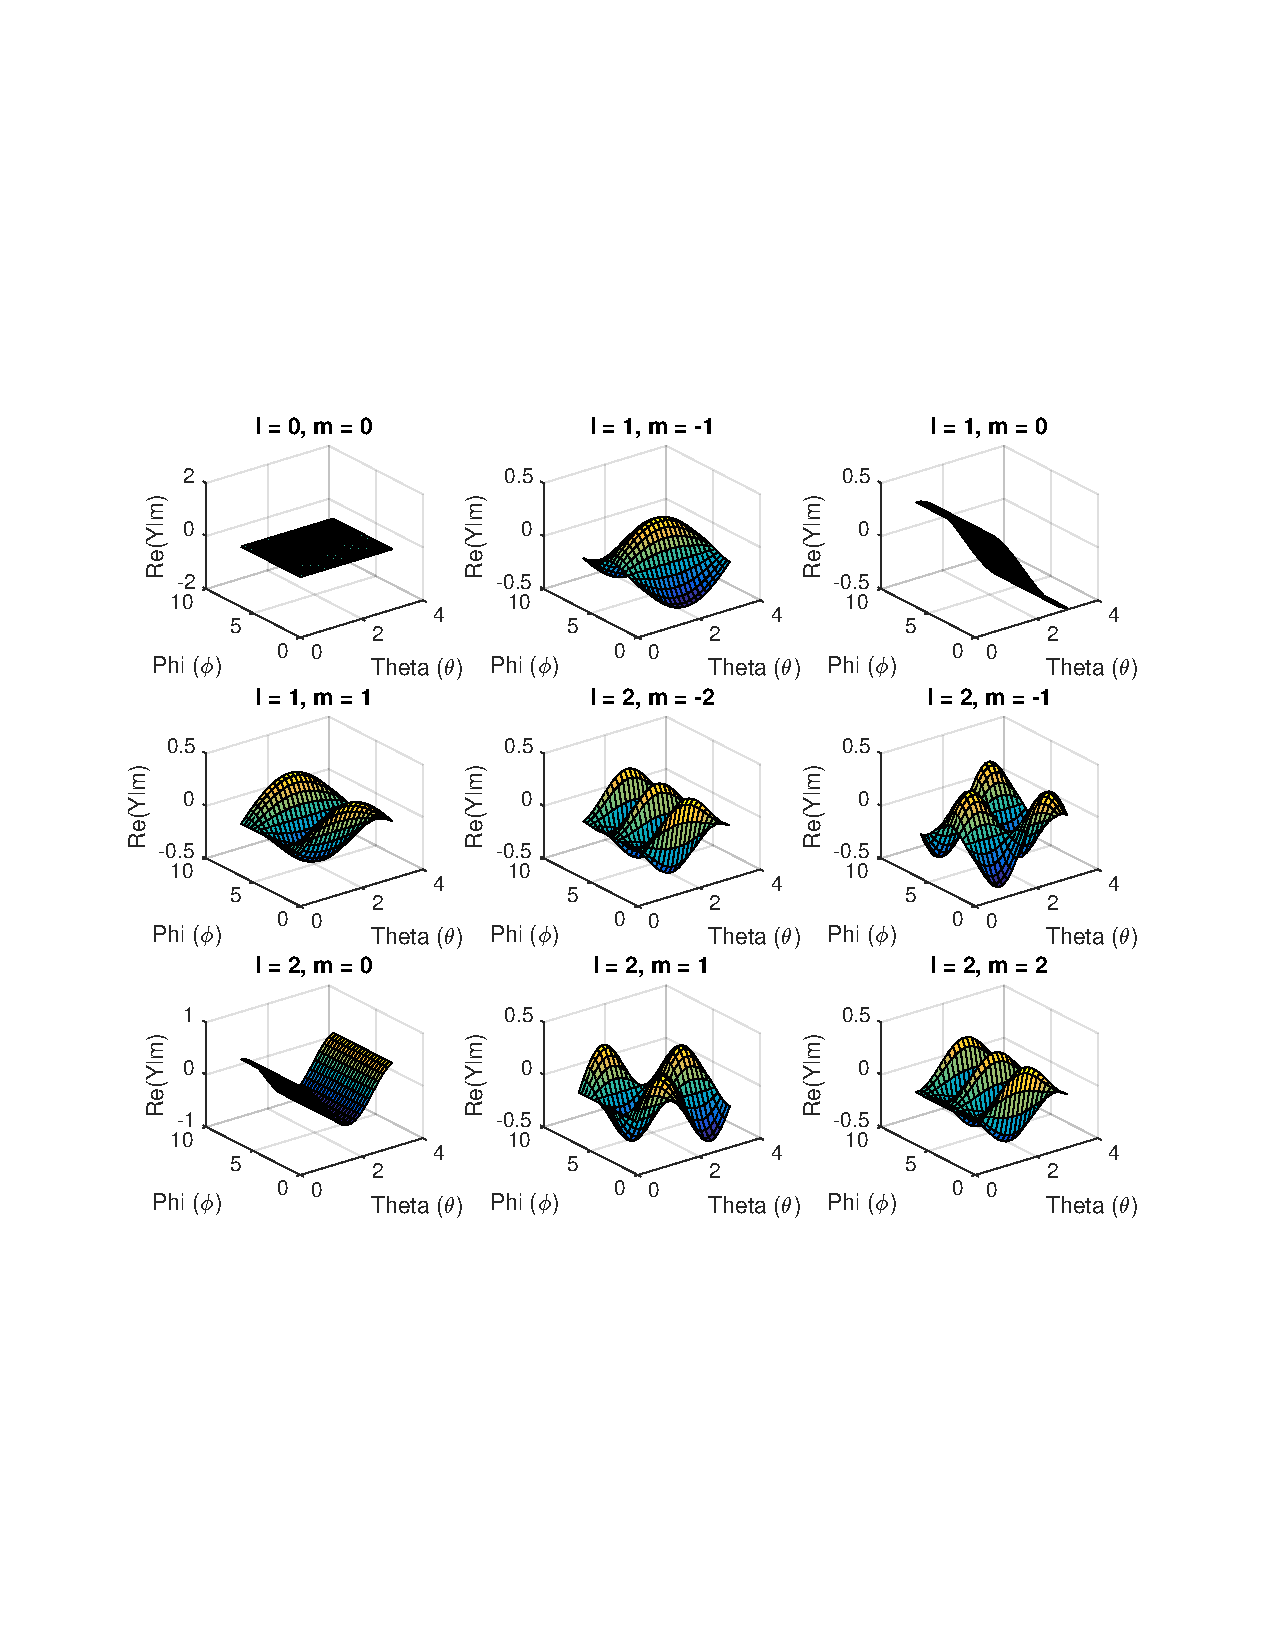
\includegraphics[width=15cm]{Real_Ylm.pdf}
  \caption{Real component of \(Y_{lm}\).}
  \label{fig:real}
\end{figure}

\clearpage
\begin{figure}[H]
  \centering
  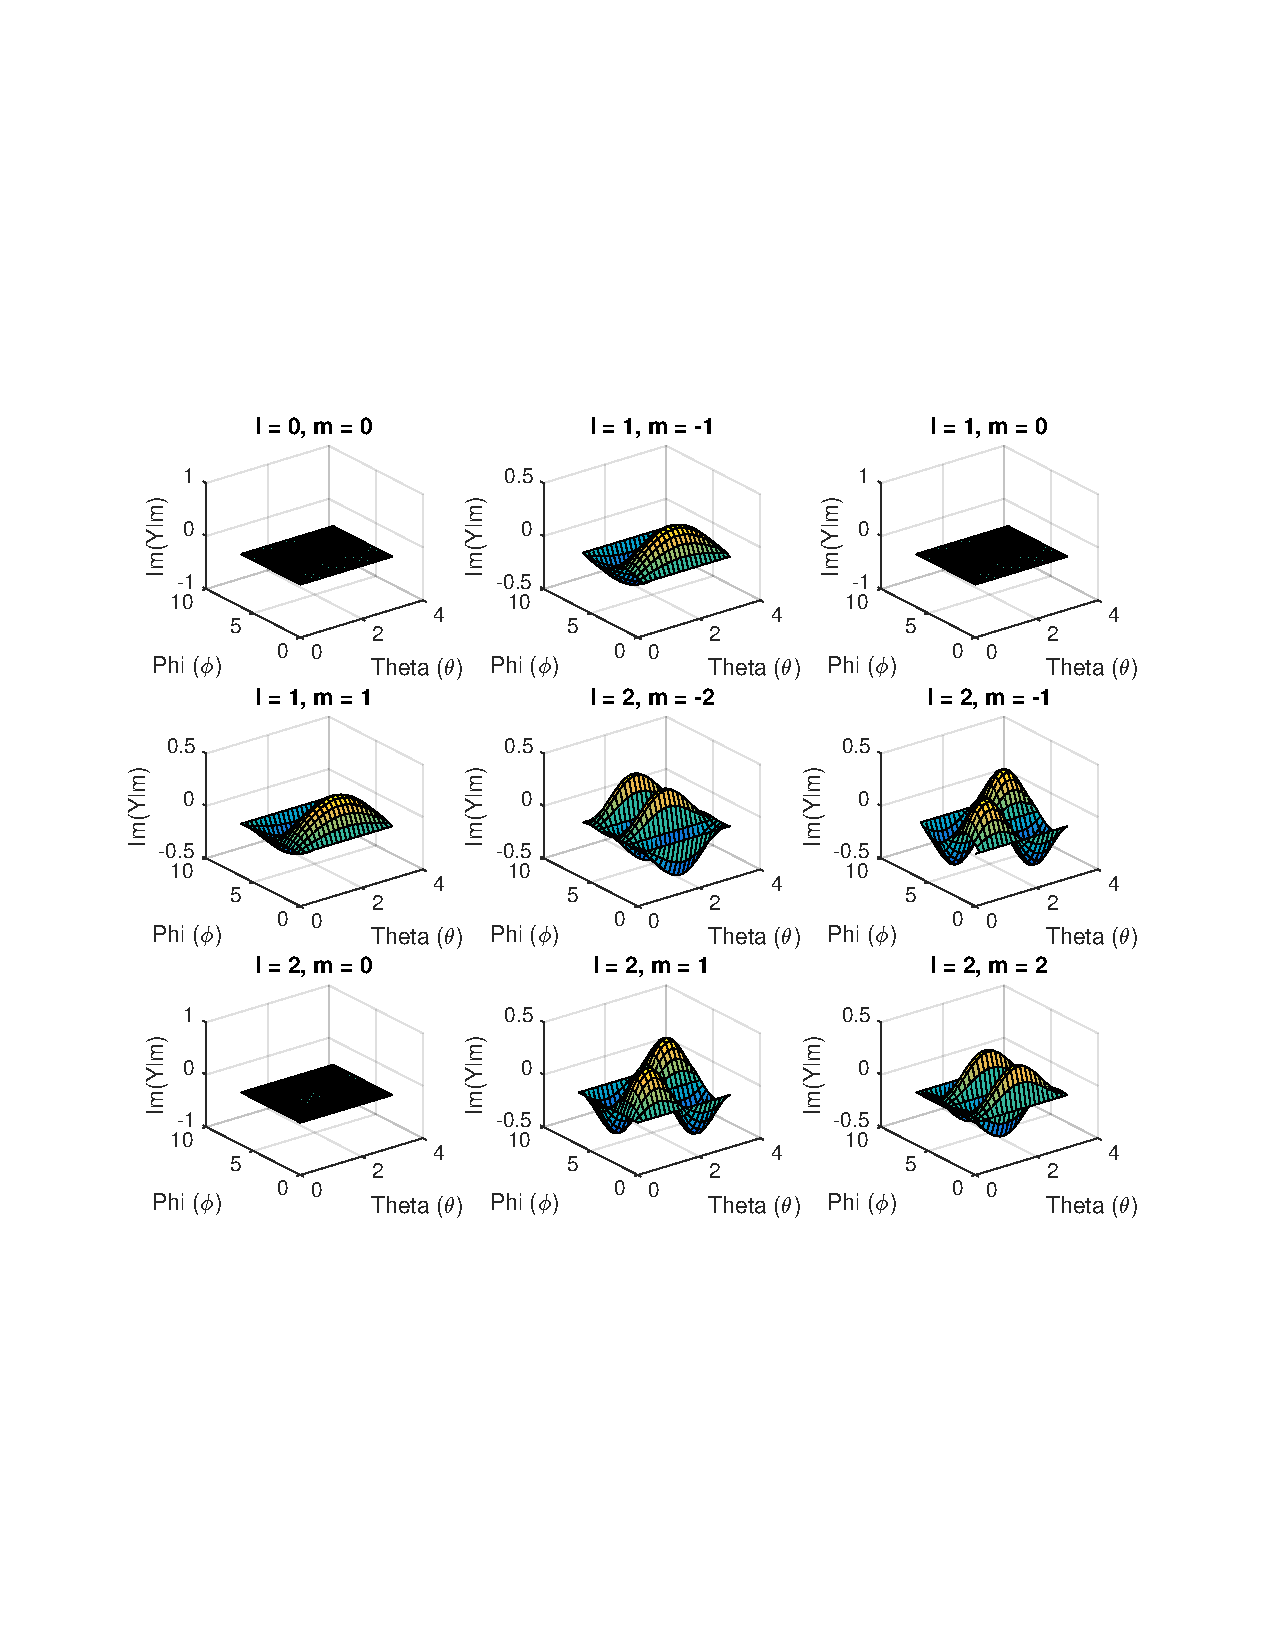
\includegraphics[width=15cm]{Imag_Ylm.pdf}
  \caption{Imaginary component of \(Y_{lm}\).}
  \label{fig:imag}
\end{figure}
\end{comment}

\clearpage
(b) 

\circled{5} Some of the major nuclear data libraries include:

\begin{enumerate}
\item ENDF (Evaluated Nuclear Data File): United States
\item JENDL (Japanese Evaluated Nuclear Data Library): Japan
\item TENDL (TALYS-based Evaluated Nuclear Data Library): (TALYS is managed by the Netherlands). TALYS is a code that contains nuclear physics to predict cross sections. Up until 2015, this library was managed in the Netherlands, but since then management has switched to France and Switzerland.
\item JEFF (Joint Evaluated Fission and Fusion File): collaboration between NEA Data Bank members
\item CENDL (Chinese Evaluated Neutron Data Library): China
\item RUSFOND: Russia
\item BROND: Russia
\end{enumerate}

\section{Appendix}
This section contains all the code used for each question. 

\subsection{Question 4}
\lstinputlisting[language=Matlab]{Q4.m}


\end{document}